%
%  Chad Conrad
%
\documentclass[12pt,fullpage]{article}
\usepackage{fullpage}
\usepackage{psfrag}                                          % LaTeX graphics tool
\usepackage{pslatex}                                         % avoids the default cmr font
\usepackage{graphicx}                                        % graphics package 
\usepackage{epsfig}                                          % figures
\usepackage{hyperref}
\usepackage{color}

\begin{document}

\noindent
{\bf Muth distribution} (from \color{blue}\url{http://www.math.wm.edu/~leemis/chart/UDR/UDR.html}\color{black})

\noindent
The shorthand $X \sim {\rm Muth}(\kappa)$ is used to indicate that the
random variable $X$ has the Muth distribution with parameter $\kappa$.
A Muth random variable $X$ with parameter $\kappa$ has probability density function 
$$
f(x) = (e ^ {\kappa x} - \kappa) e ^ {[-\frac{e ^ {\kappa x}}{\kappa} +\kappa x +\frac{1}{\kappa}]} \qquad \qquad x > 0
$$
for $0<\kappa \leq 1.$
The probability density function for three different values of $\kappa$ is illustrated below.
{\begin{figure}[h!]
\begin{center}
\psfrag{lab1}{$\kappa = 0.2$}
\psfrag{lab2}{$\kappa = 0.5$}
\psfrag{lab3}{$\kappa = 1.0$}
\psfrag{labx}{$x$}
\psfrag{labf}{$f(x)$}
\includegraphics[width=3.2in]{MuthPlot.ps}
\end{center}
\end{figure}}\\
The cumulative distribution function on
the support of $X$ is
$$
F(x) = P(X \le x) = 1 - e ^ {\left[-\frac{e ^ {\kappa x}}{\kappa} + \kappa x + \frac{1}{\kappa} \right]} \qquad \qquad x > 0.
$$
The survivor function on the support of $X$ is
$$
S(x) = P(X \ge x) = e ^ {\left[-\frac{e ^ {\kappa x}}{\kappa} +\kappa x + \frac{1}{\kappa} \right]} \qquad \qquad x > 0.
$$
The hazard function on the support of $X$ is
$$
h(x) = \frac{f(x)}{S(x)} = e ^ {\kappa x} -\kappa \qquad \qquad x > 0.
$$
The cumulative hazard function on the support of $X$ is
$$
H(x) = - \ln S(x) = \frac{e ^ {\kappa x}}{\kappa} -\kappa x - \frac{1}{\kappa} \qquad \qquad x > 0.
$$
The inverse distribution function, median, moment generating function and characteristic function of $X$ are not mathematically tractable.\\
\\
The population mean is
$$
E[X] = 1. \qquad \qquad 
$$

\vspace{0.1in}

\newpage
\noindent
{\bf APPL verification:}
The APPL statements
\begin{verbatim}
X := MuthRV(kappa);
CDF(X);
SF(X);
HF(X);
CHF(X);
Mean(X);
\end{verbatim}
verify the verify the cumulative distribution, survivor function, hazard function, cumulative hazard function, population mean.

\end{document}
